\chapter{Umsetzung und Ergebnisse}
\label{cha:umsetzung}
Um die bestmögliche Dokumentation des Systemaufbaus sicherstellen zu können, dürfen die Vorbereitungen, auf die Aufgabe, nicht unterschätzt werden. Diese lassen sich in zwei große Teile aufgeteilen. Der wichtigere von beiden Schritten ist die sorgfältige Auswahl eines passenden Tools zur Erstellung der Dokumentation. Aspekte wie Benutzerfreundlichkeit, Funktionen die erfüllt werden, Betriebssystemkompatibilitäten und Kosten spielen hier eine große Rolle. Um diese Auswahl mit genügend Sorgfalt zu treffen wird folgendes Vorgehen angewandt:

Es werden verschiedene CAD-Softwareprogramm recherchiert und evaluiert. Die Funktionen stehen hier an erster Stelle. Das Programm muss in der Lage sein, Stromlaufpläne und Bestückungspläne erstellen zu können. An nächster Stelle stehen die Kosten, die für das Programm abgerufen werden. Da das Projekt ein begrenztes Budget hat sollen diese möglichst gering gehalten werden. Wichtig zu beachten ist hierbei jedoch, dass die Kosten im Verhältnis zur gebotenen Leistung des Programms stehen müssen. Die Programme \textit{Autodesk Fusion 360} und \textit{EPlan} sind jeweils sehr vielversprechend. Die Nutzerfreundlichkeit ist in beiden Programmen gleichermaßen gegen. Entschieden wird sich für Autodesk Fusion 360, da EPlan über keine macOS kompatibilität verfügt.

Im nächsten Schritt der Vorbereitung muss eine tiefgreifende und umfassende Einarbeitung in das Programm durchgeführt werden. Hier wird ein besonderes Augenmerk auf die Aspekte Stromlaufplanerstellung, Bestückungsplanerstellung, Bibliothekerstellung und die dazugehörige Erstellung neuer Bauteile sowie die Programm-Projekt-Struktur gelegt.



% Linke Hälfte der A3-Seite
%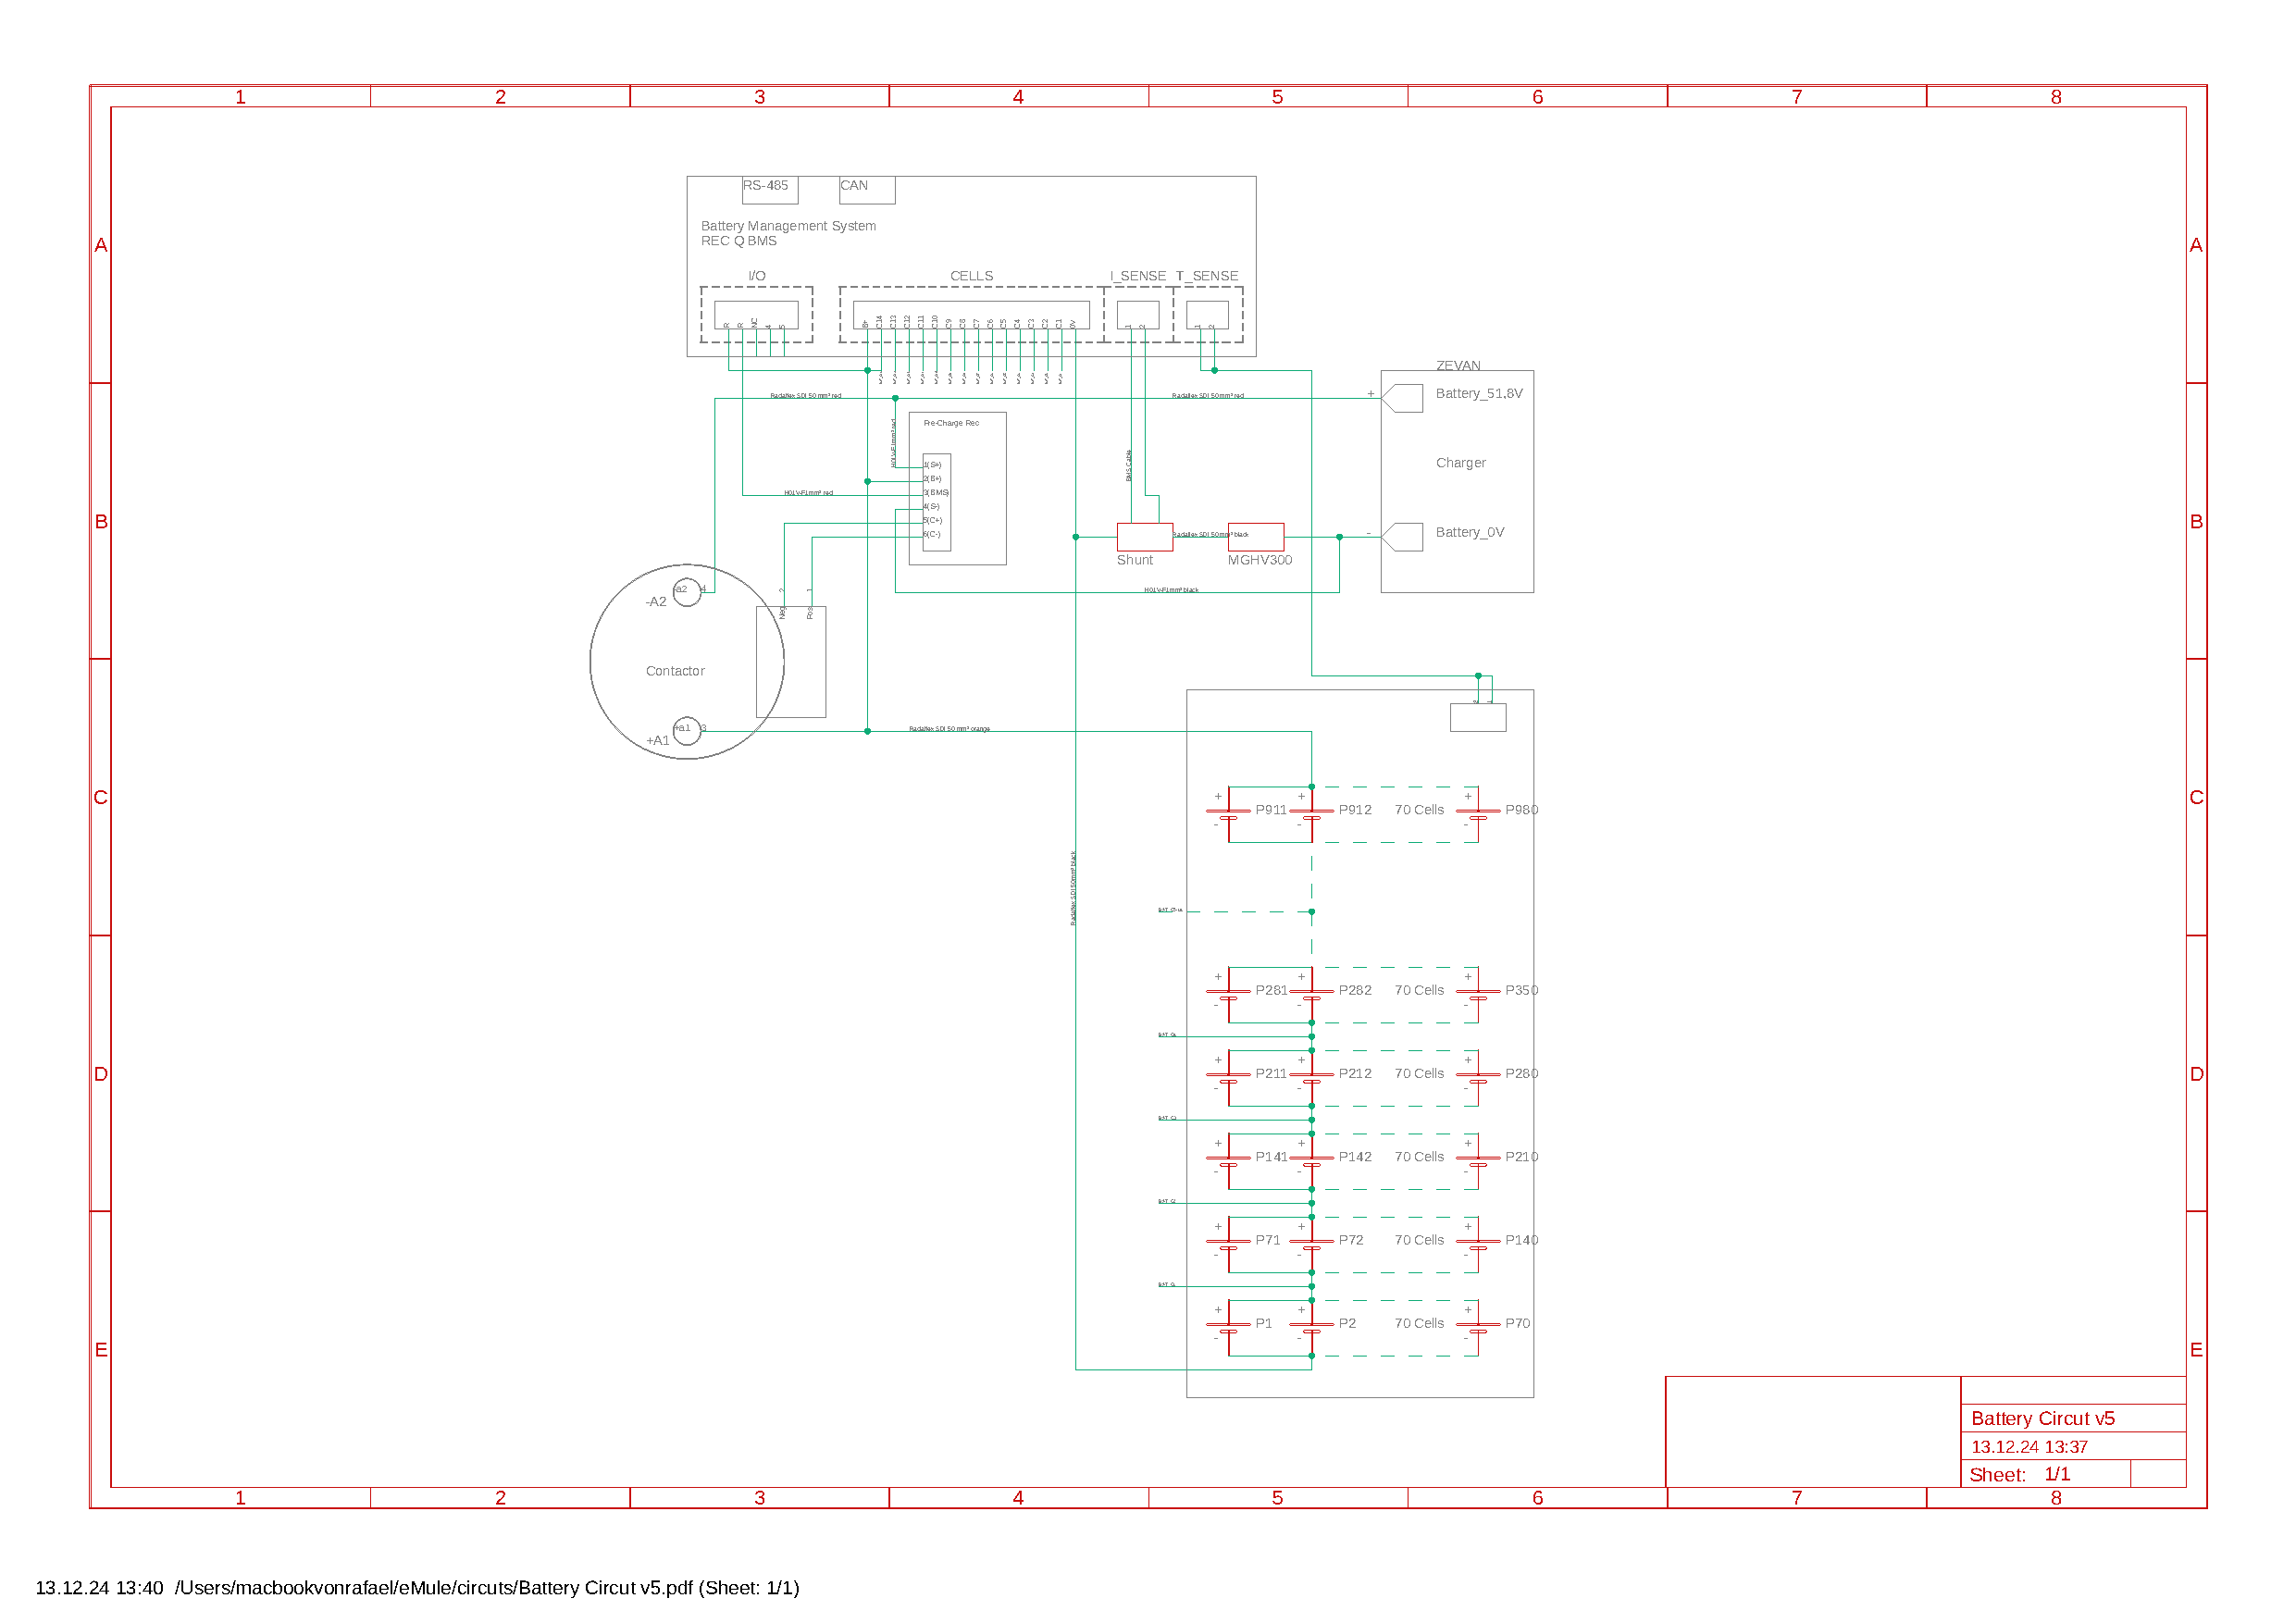
\includepdf[pages=1, trim=0cm 0cm 21cm 0cm, clip]{circuts/Battery Circut v5.pdf}

% Rechte Hälfte der A3-Seite
%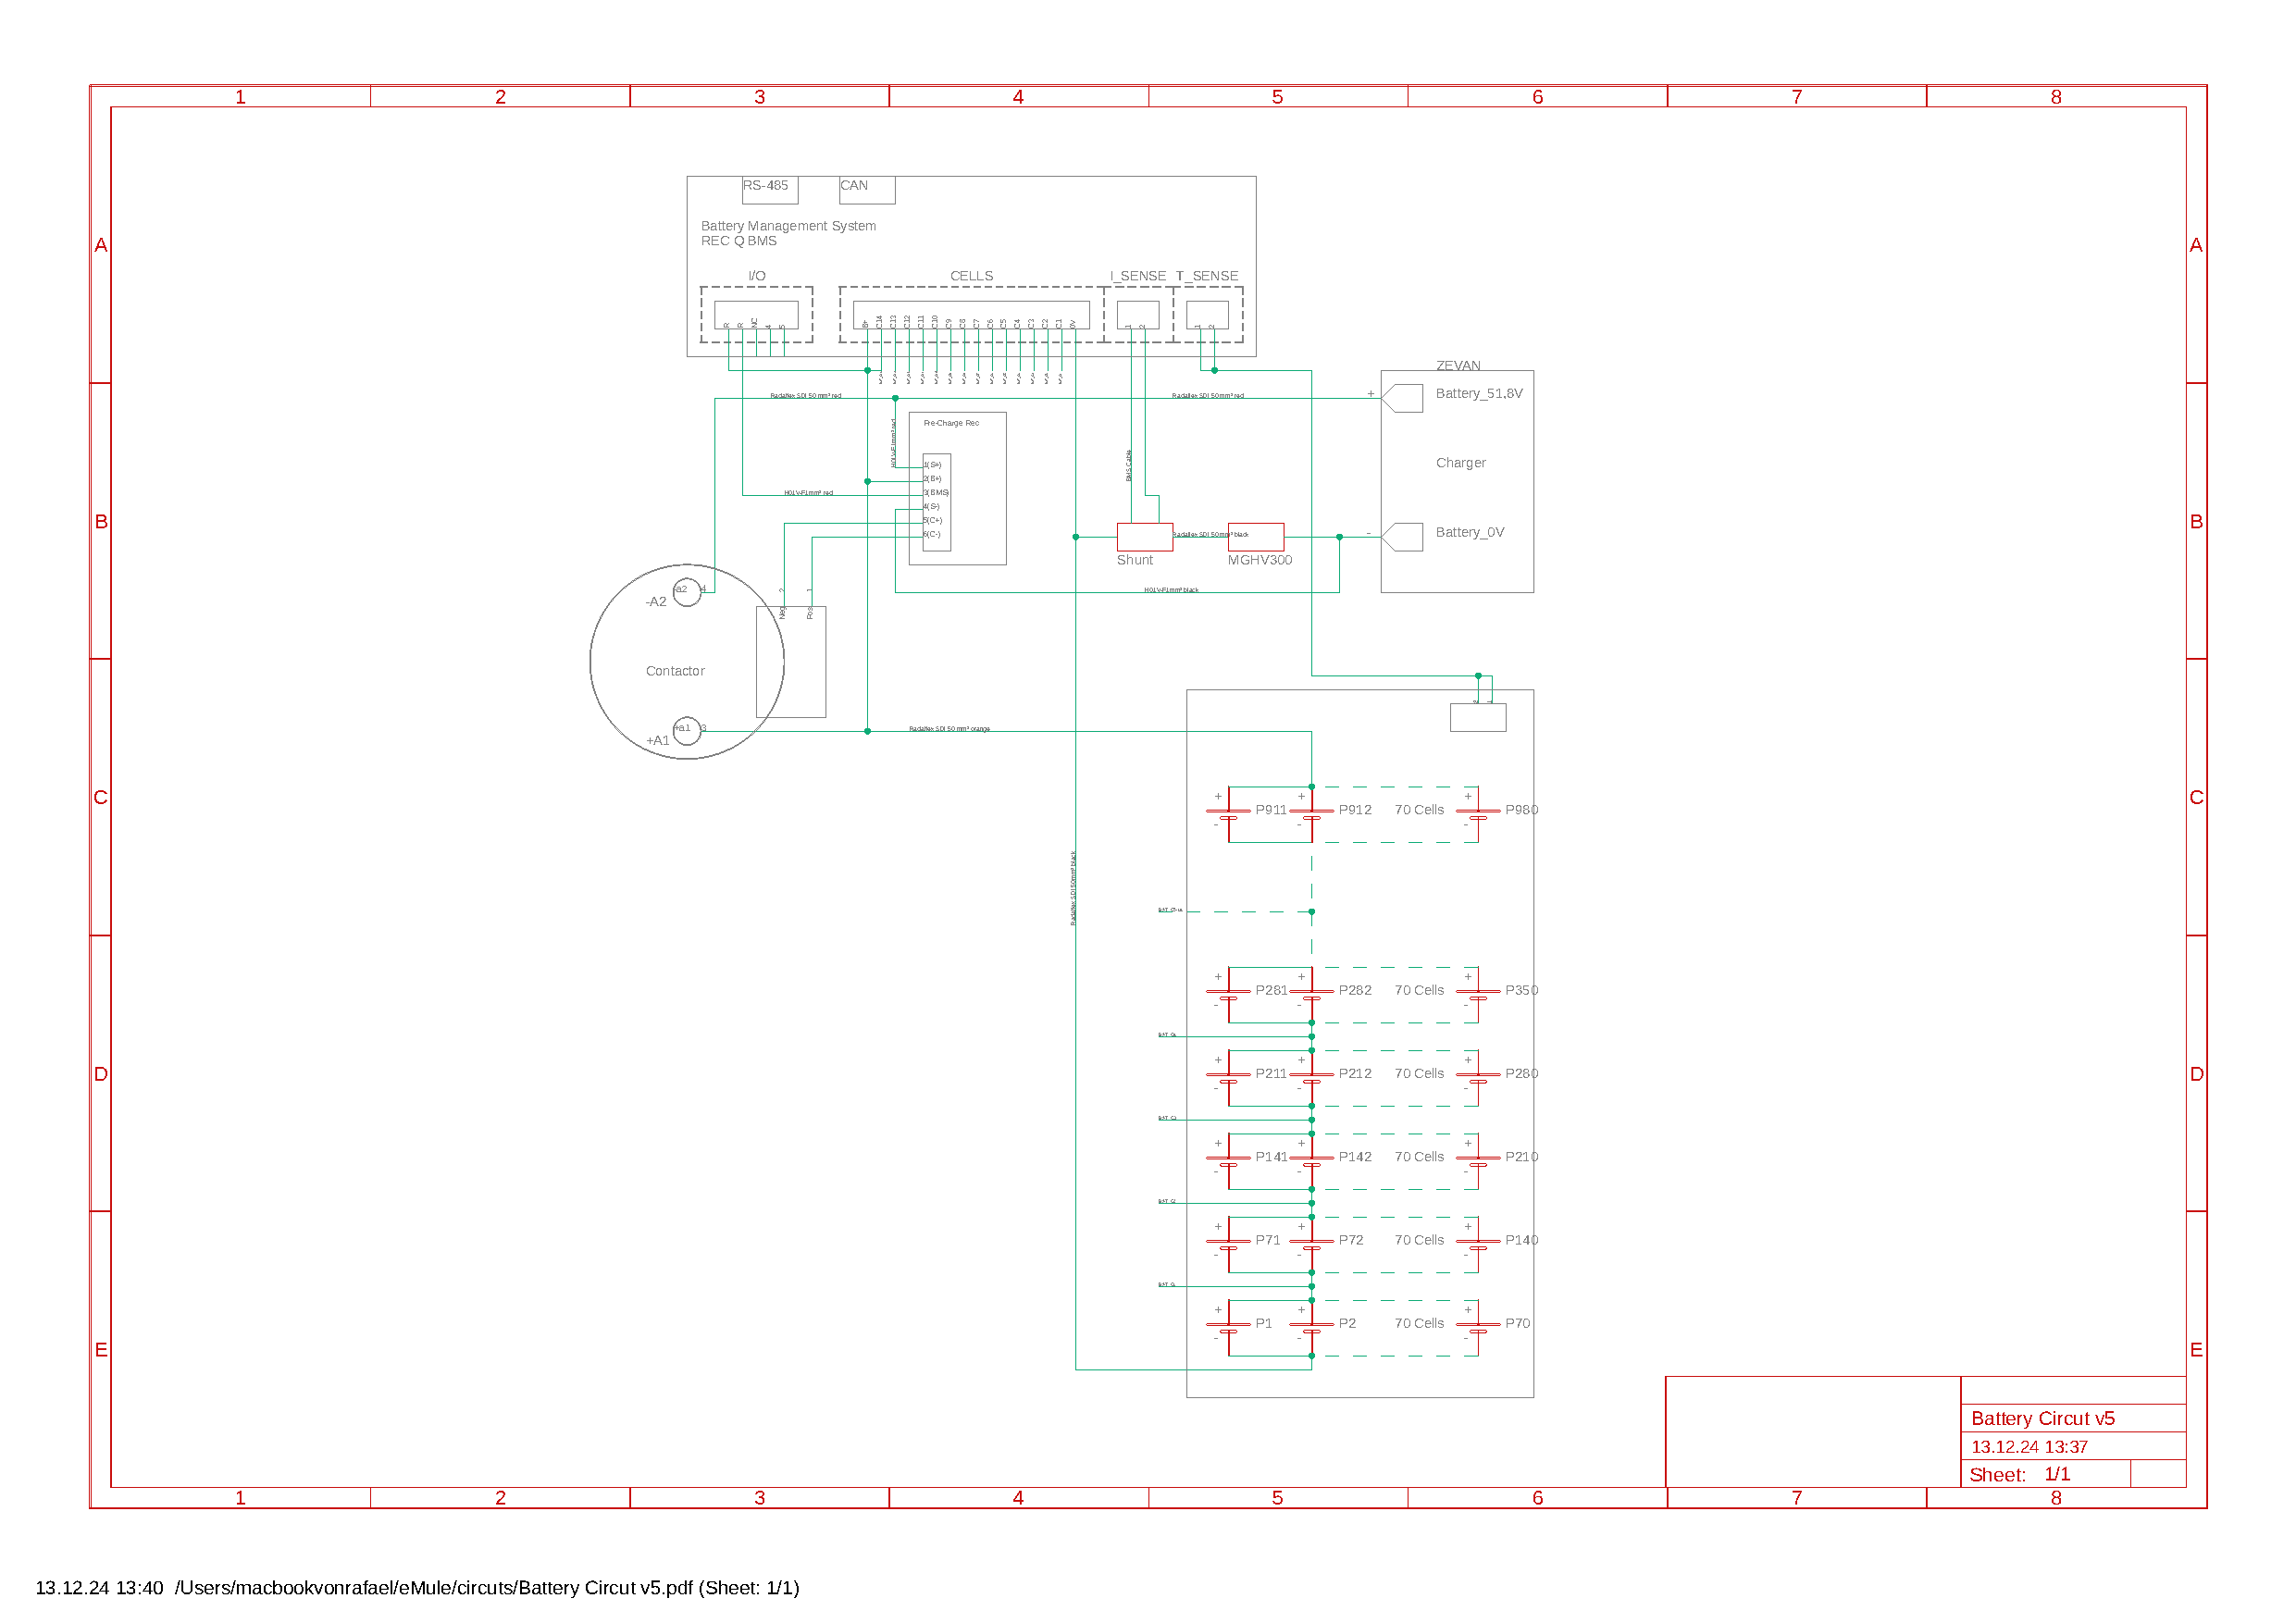
\includepdf[pages=1, trim=21cm 0cm 0cm 0cm, clip]{circuts/Battery Circut v5.pdf}

%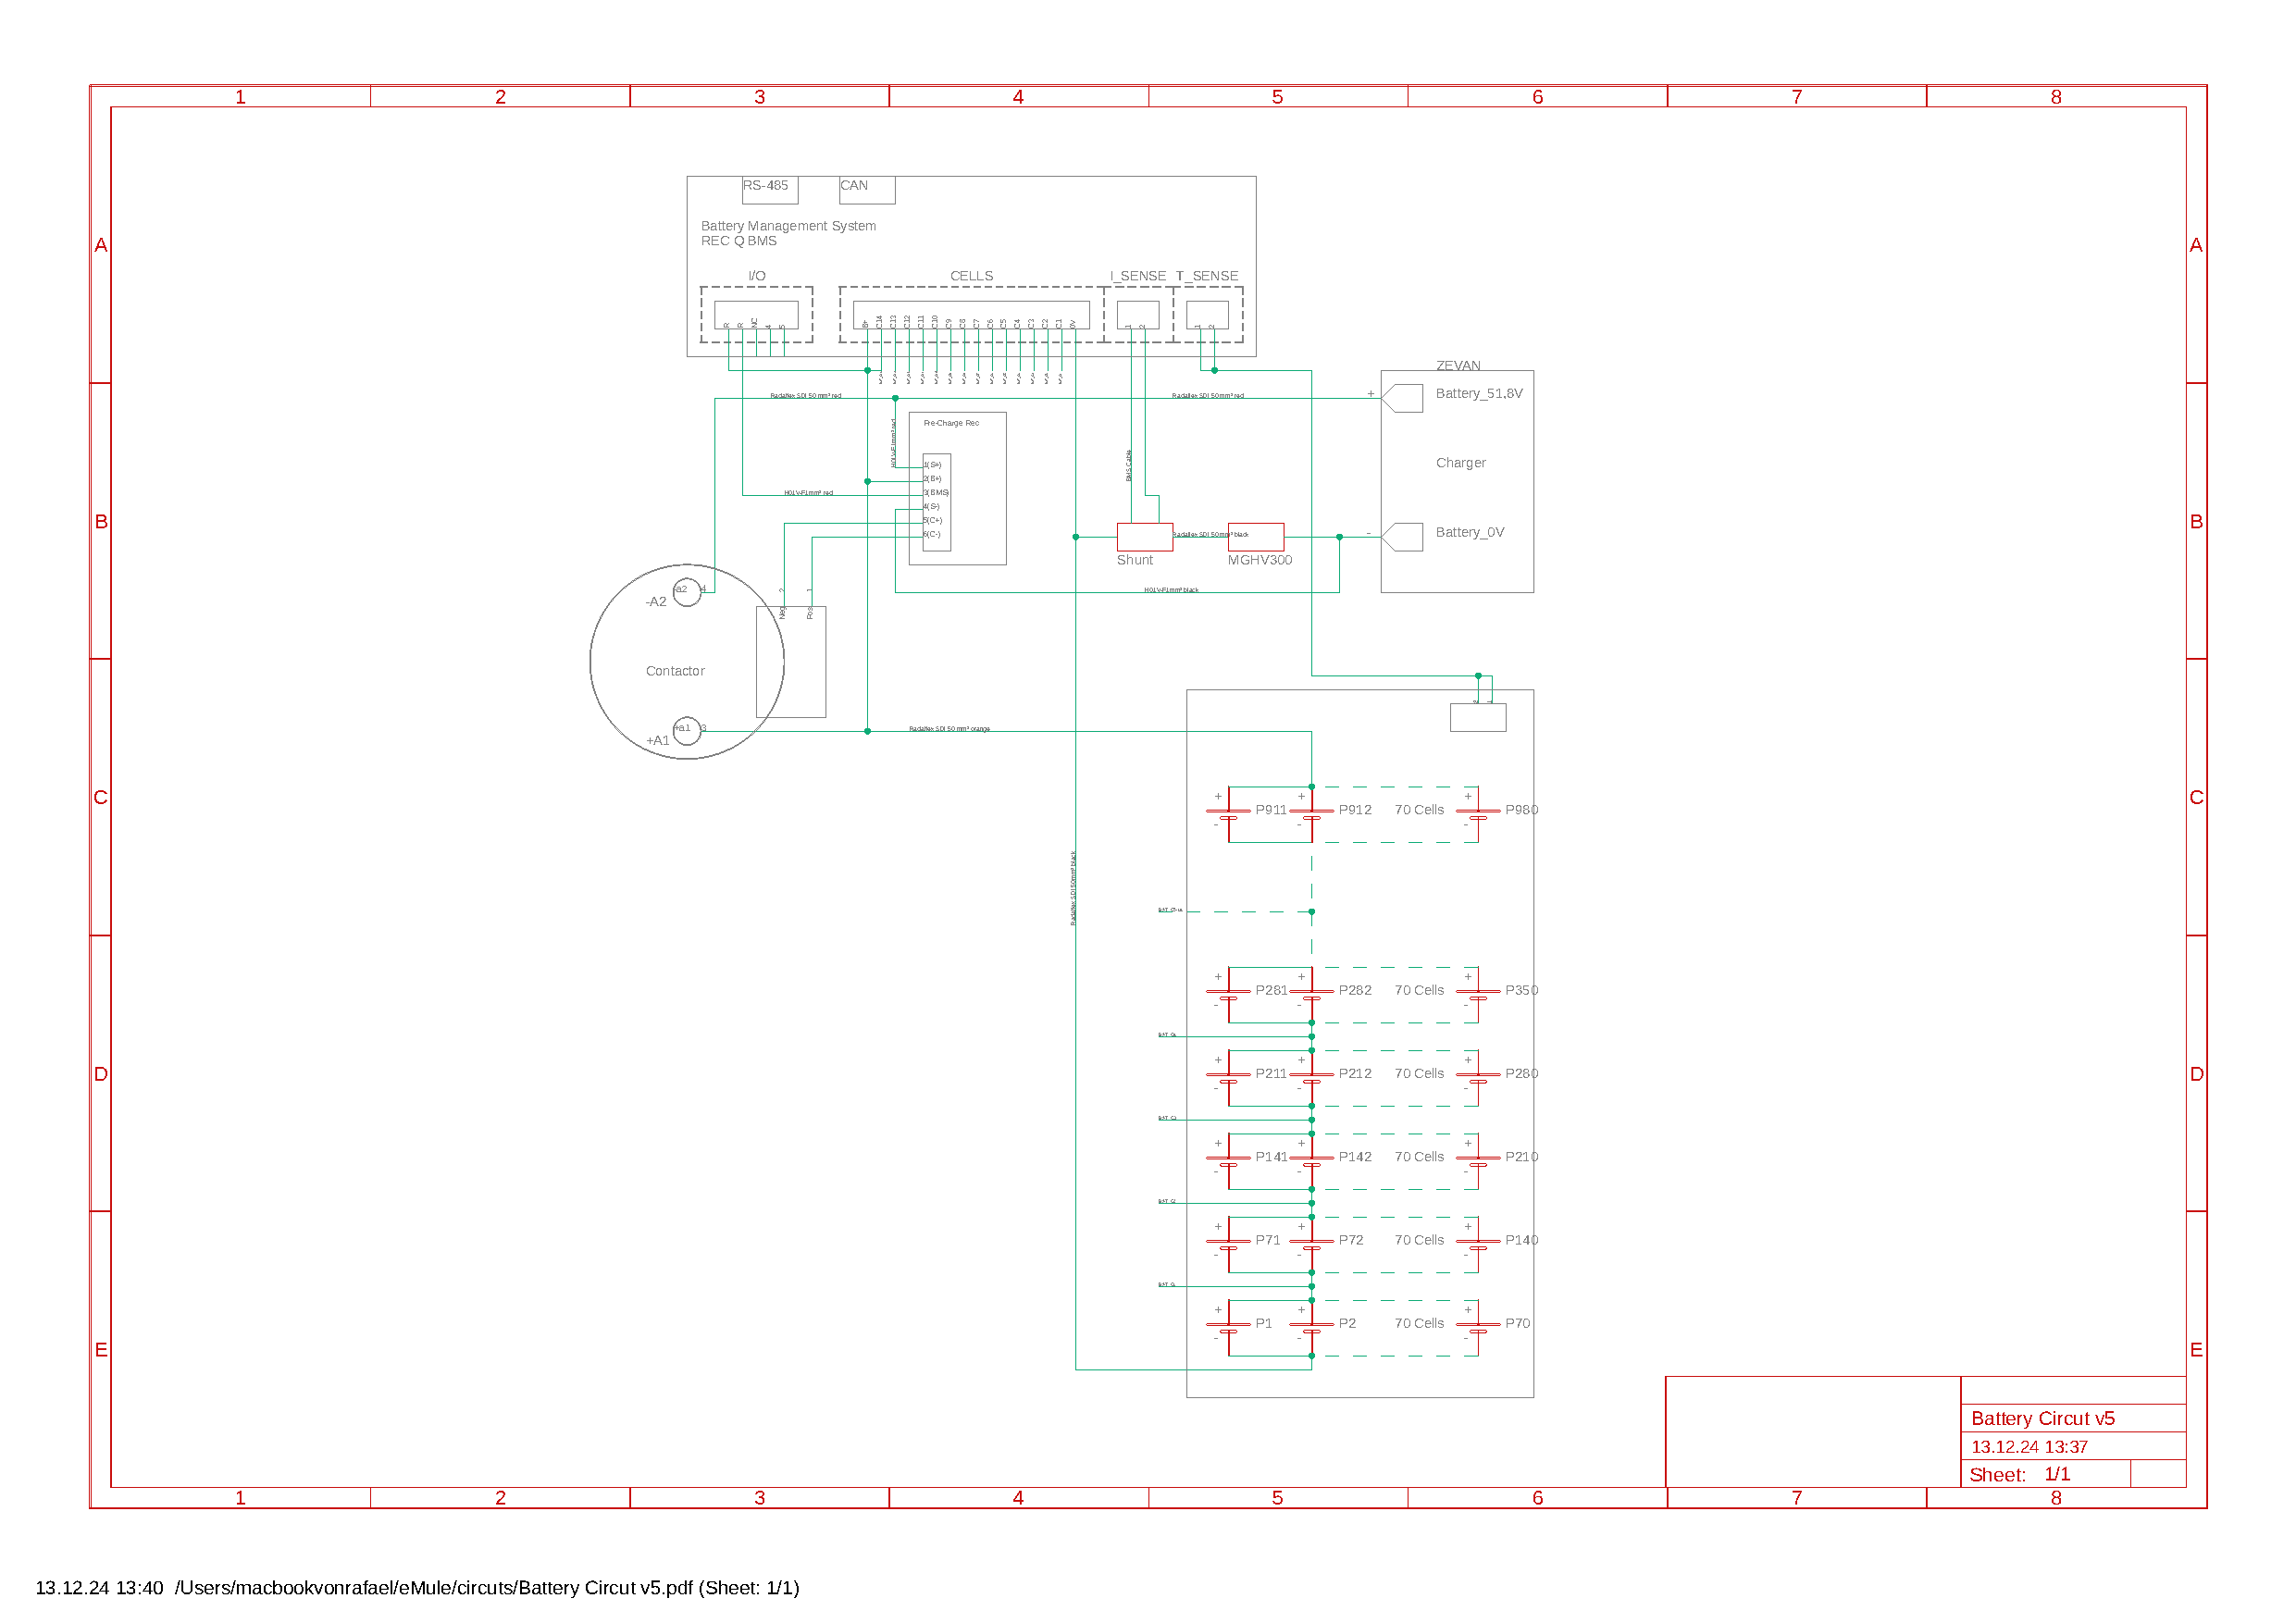
\includepdf[pages=1, angle=90, fitpaper=true]{circuts/Battery Circut v5.pdf}

\section*{Stromlaufplan Battery Circuit}
Für die Erstellung des \textit{Battery Circuit} Stromlaufplans nach festgelegter Norm und aktuellem Verbaustand wird der vorliegende Plan zunächst ausgedruckt. Im ersten Schritt wird dieser Stromlaufplan systematisch auf Unstimmigkeiten, wie fehlende Verbindungen oder unklare Symbolik, überprüft. Gefundene Fehler werden im nächsten Schritt markiert und anschließend korrigiert, wobei die Einhaltung elektrotechnischer Standards gewährleistet wird. Zudem erfolgt eine Layoutanpassung zur Verbesserung der Übersichtlichkeit. Im letzten Schritt muss herausgefunden werden, nach welcher Norm der Stromlaufplan erstellt wurde. Diese Norm muss recherchiert und in die von uns gewählte DIN EN 60617 Norm \glqq übersetzt\grqq {} werden. Der überarbeitete Stromlaufplan wird abschließend mit Autodesk Fusion 360 in ein DIN-A3-Format übertragen. Dabei werden Titelblock und Legende integriert, um die Professionalität und Lesbarkeit sicherzustellen.

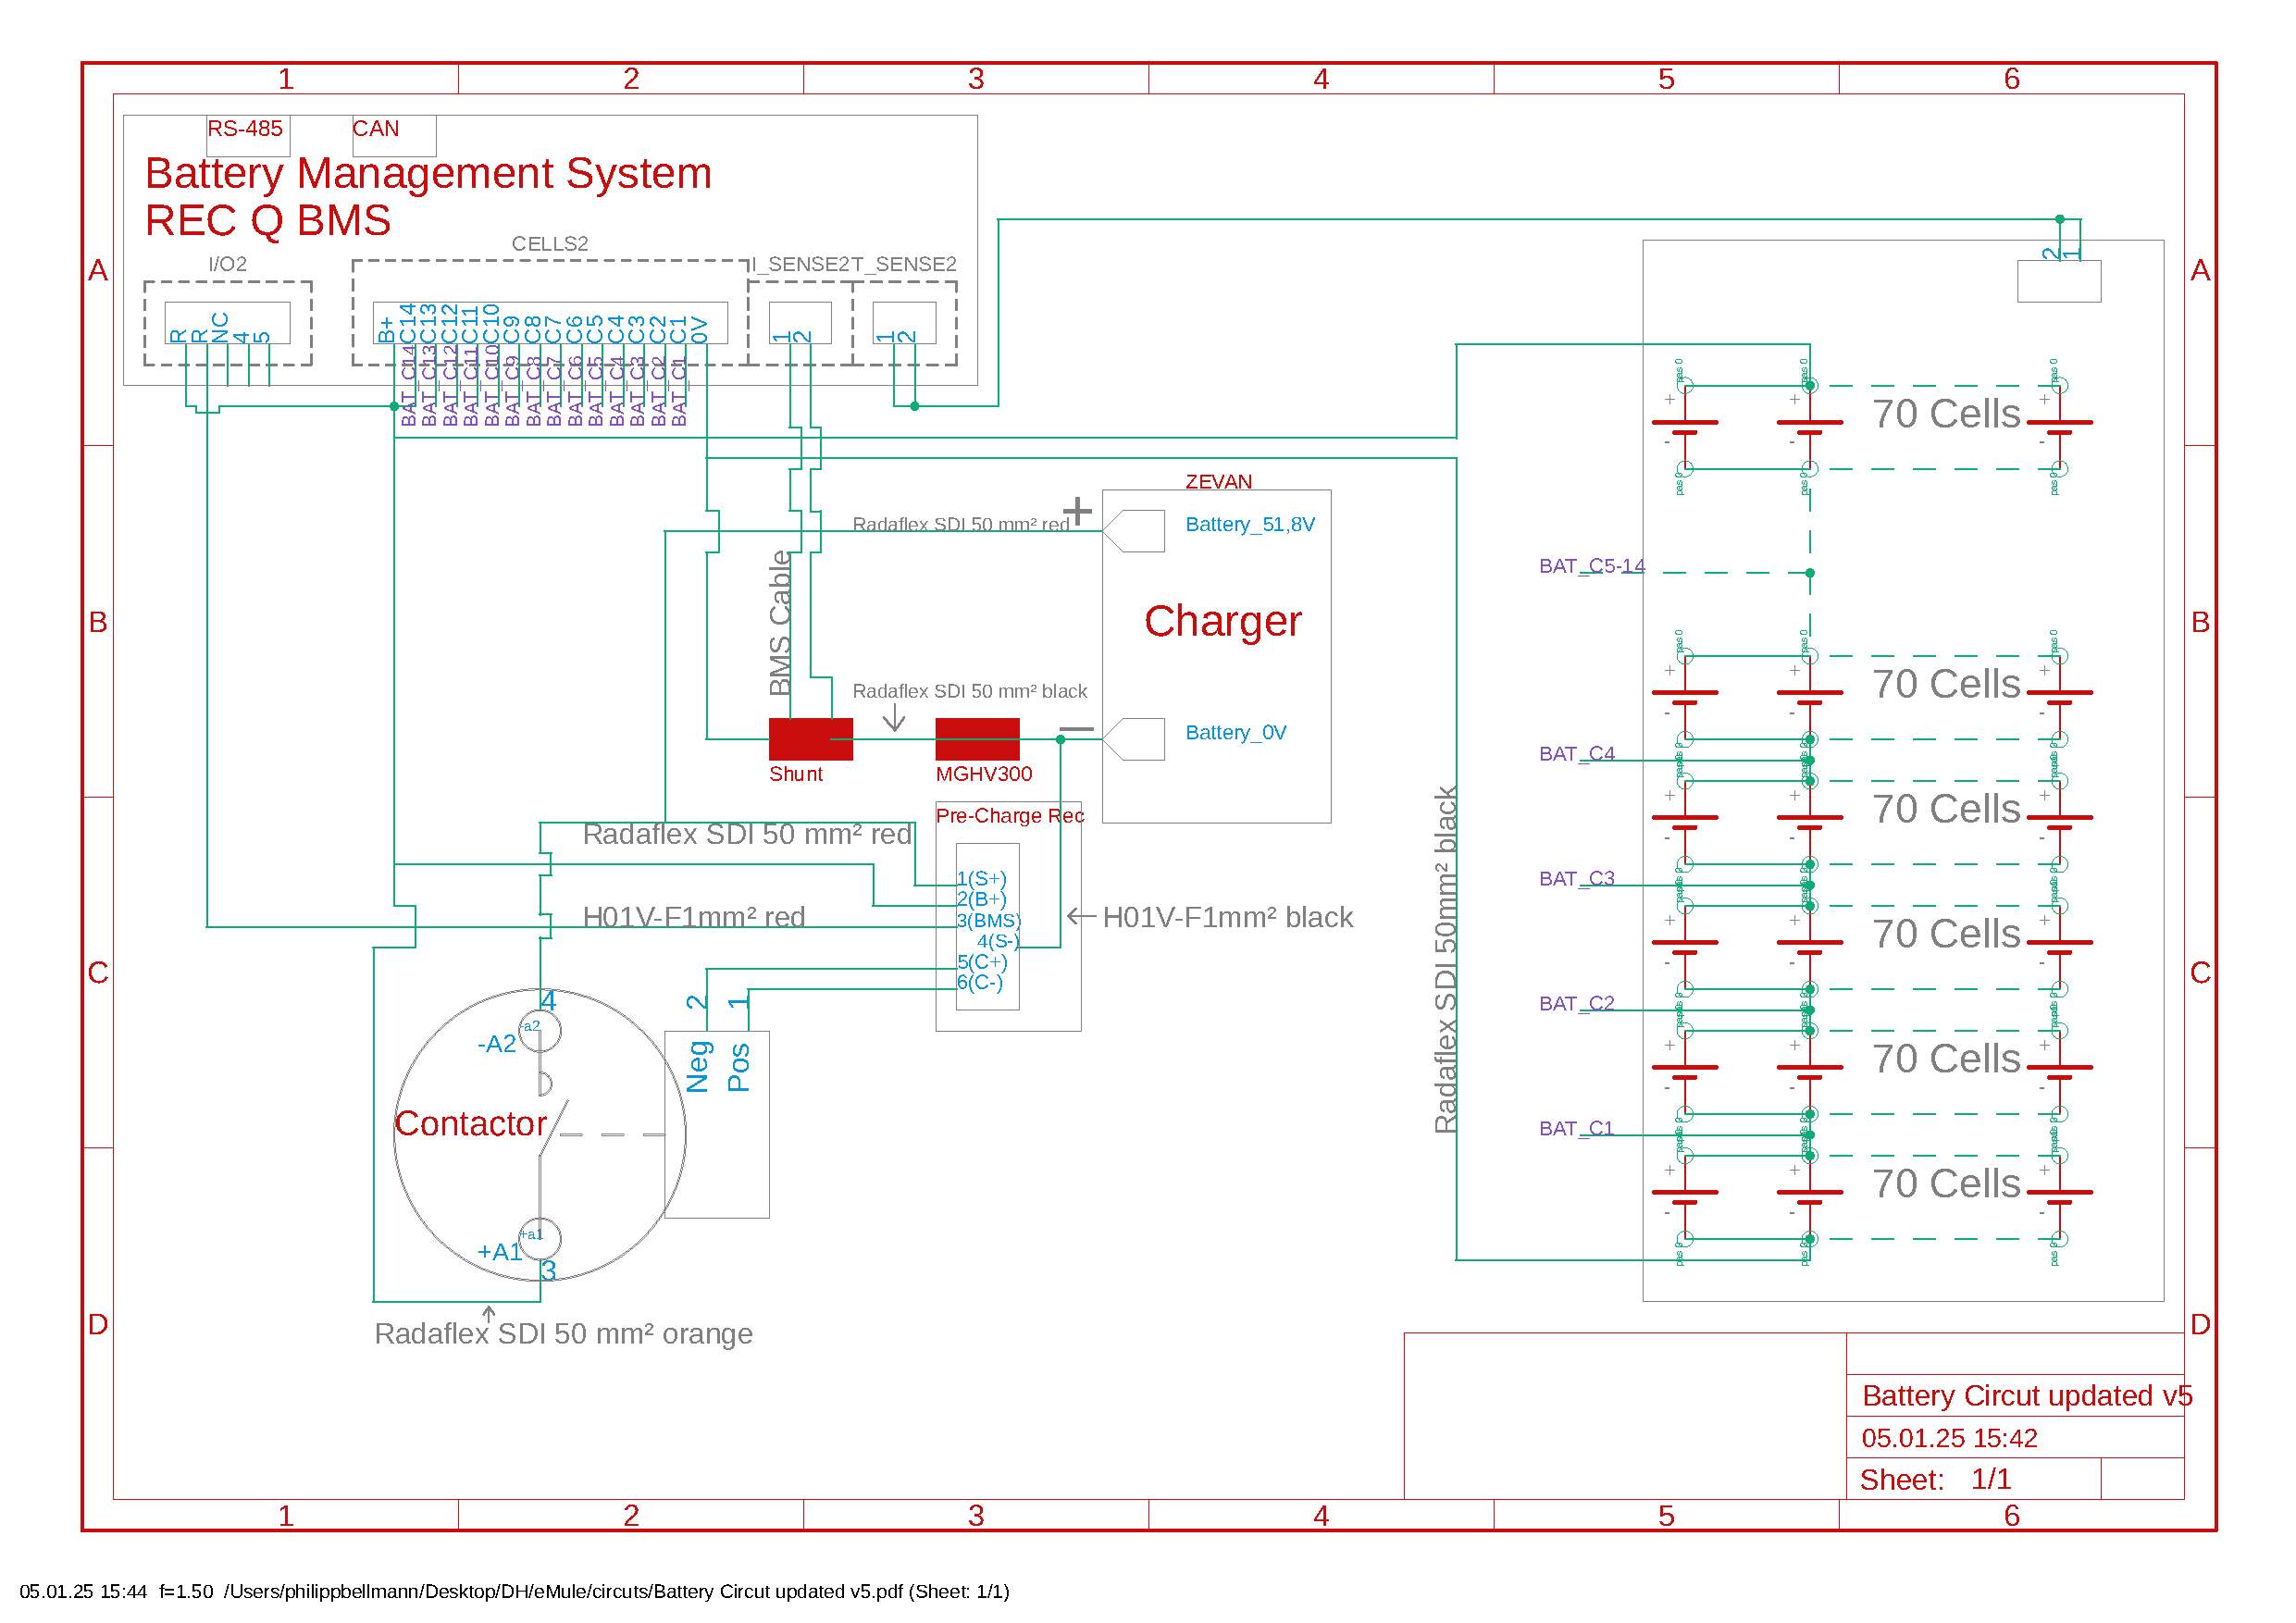
\includepdf[pages=1, fitpaper=true, pagecommand={%
	\thispagestyle{empty} % Entfernt Seitenzahlen und Kopfzeilen
	\begin{center}
		\vspace*{-5cm} % Verschiebt die Caption um 2 cm nach oben
		\hspace{10cm} % Verschiebt die Caption um 10 cm nach rechts
		\captionof{figure}{Schaltplan des Battery Circuits} % Fügt die Caption ein
		\label{fig:battery_circuit} % Für Querverweise
	\end{center}
}]{circuts/Battery Circut updated.pdf}
\addtocounter{page}{1} % Seitenzähler korrekt erhöhen

% Zweite PDF: Motor Controller
\section*{Stromlaufplan Motor Controller}
Für die Erstellung des \textit{Motor Controller} Stromlaufplans nach festgelegter Norm und aktuellem Verbaustand wird der vorliegende Plan zunächst ausgedruckt. Im ersten Schritt wird dieser Stromlaufplan systematisch auf Unstimmigkeiten, wie fehlende Verbindungen oder unklare Symbolik, überprüft. Gefundene Fehler werden im nächsten Schritt markiert und anschließend korrigiert, wobei die Einhaltung elektrotechnischer Standards gewährleistet wird. Zudem erfolgt eine Layoutanpassung zur Verbesserung der Übersichtlichkeit. Im letzten Schritt muss herausgefunden werden, nach welcher Norm der Stromlaufplan erstellt wurde. Diese Norm muss recherchiert und in die von uns gewählte DIN EN 60617 Norm \glqq übersetzt\grqq {} werden. Der überarbeitete Stromlaufplan wird abschließend mit Autodesk Fusion 360 in ein DIN-A3-Format übertragen. Dabei werden Titelblock und Legende integriert, um die Professionalität und Lesbarkeit sicherzustellen.

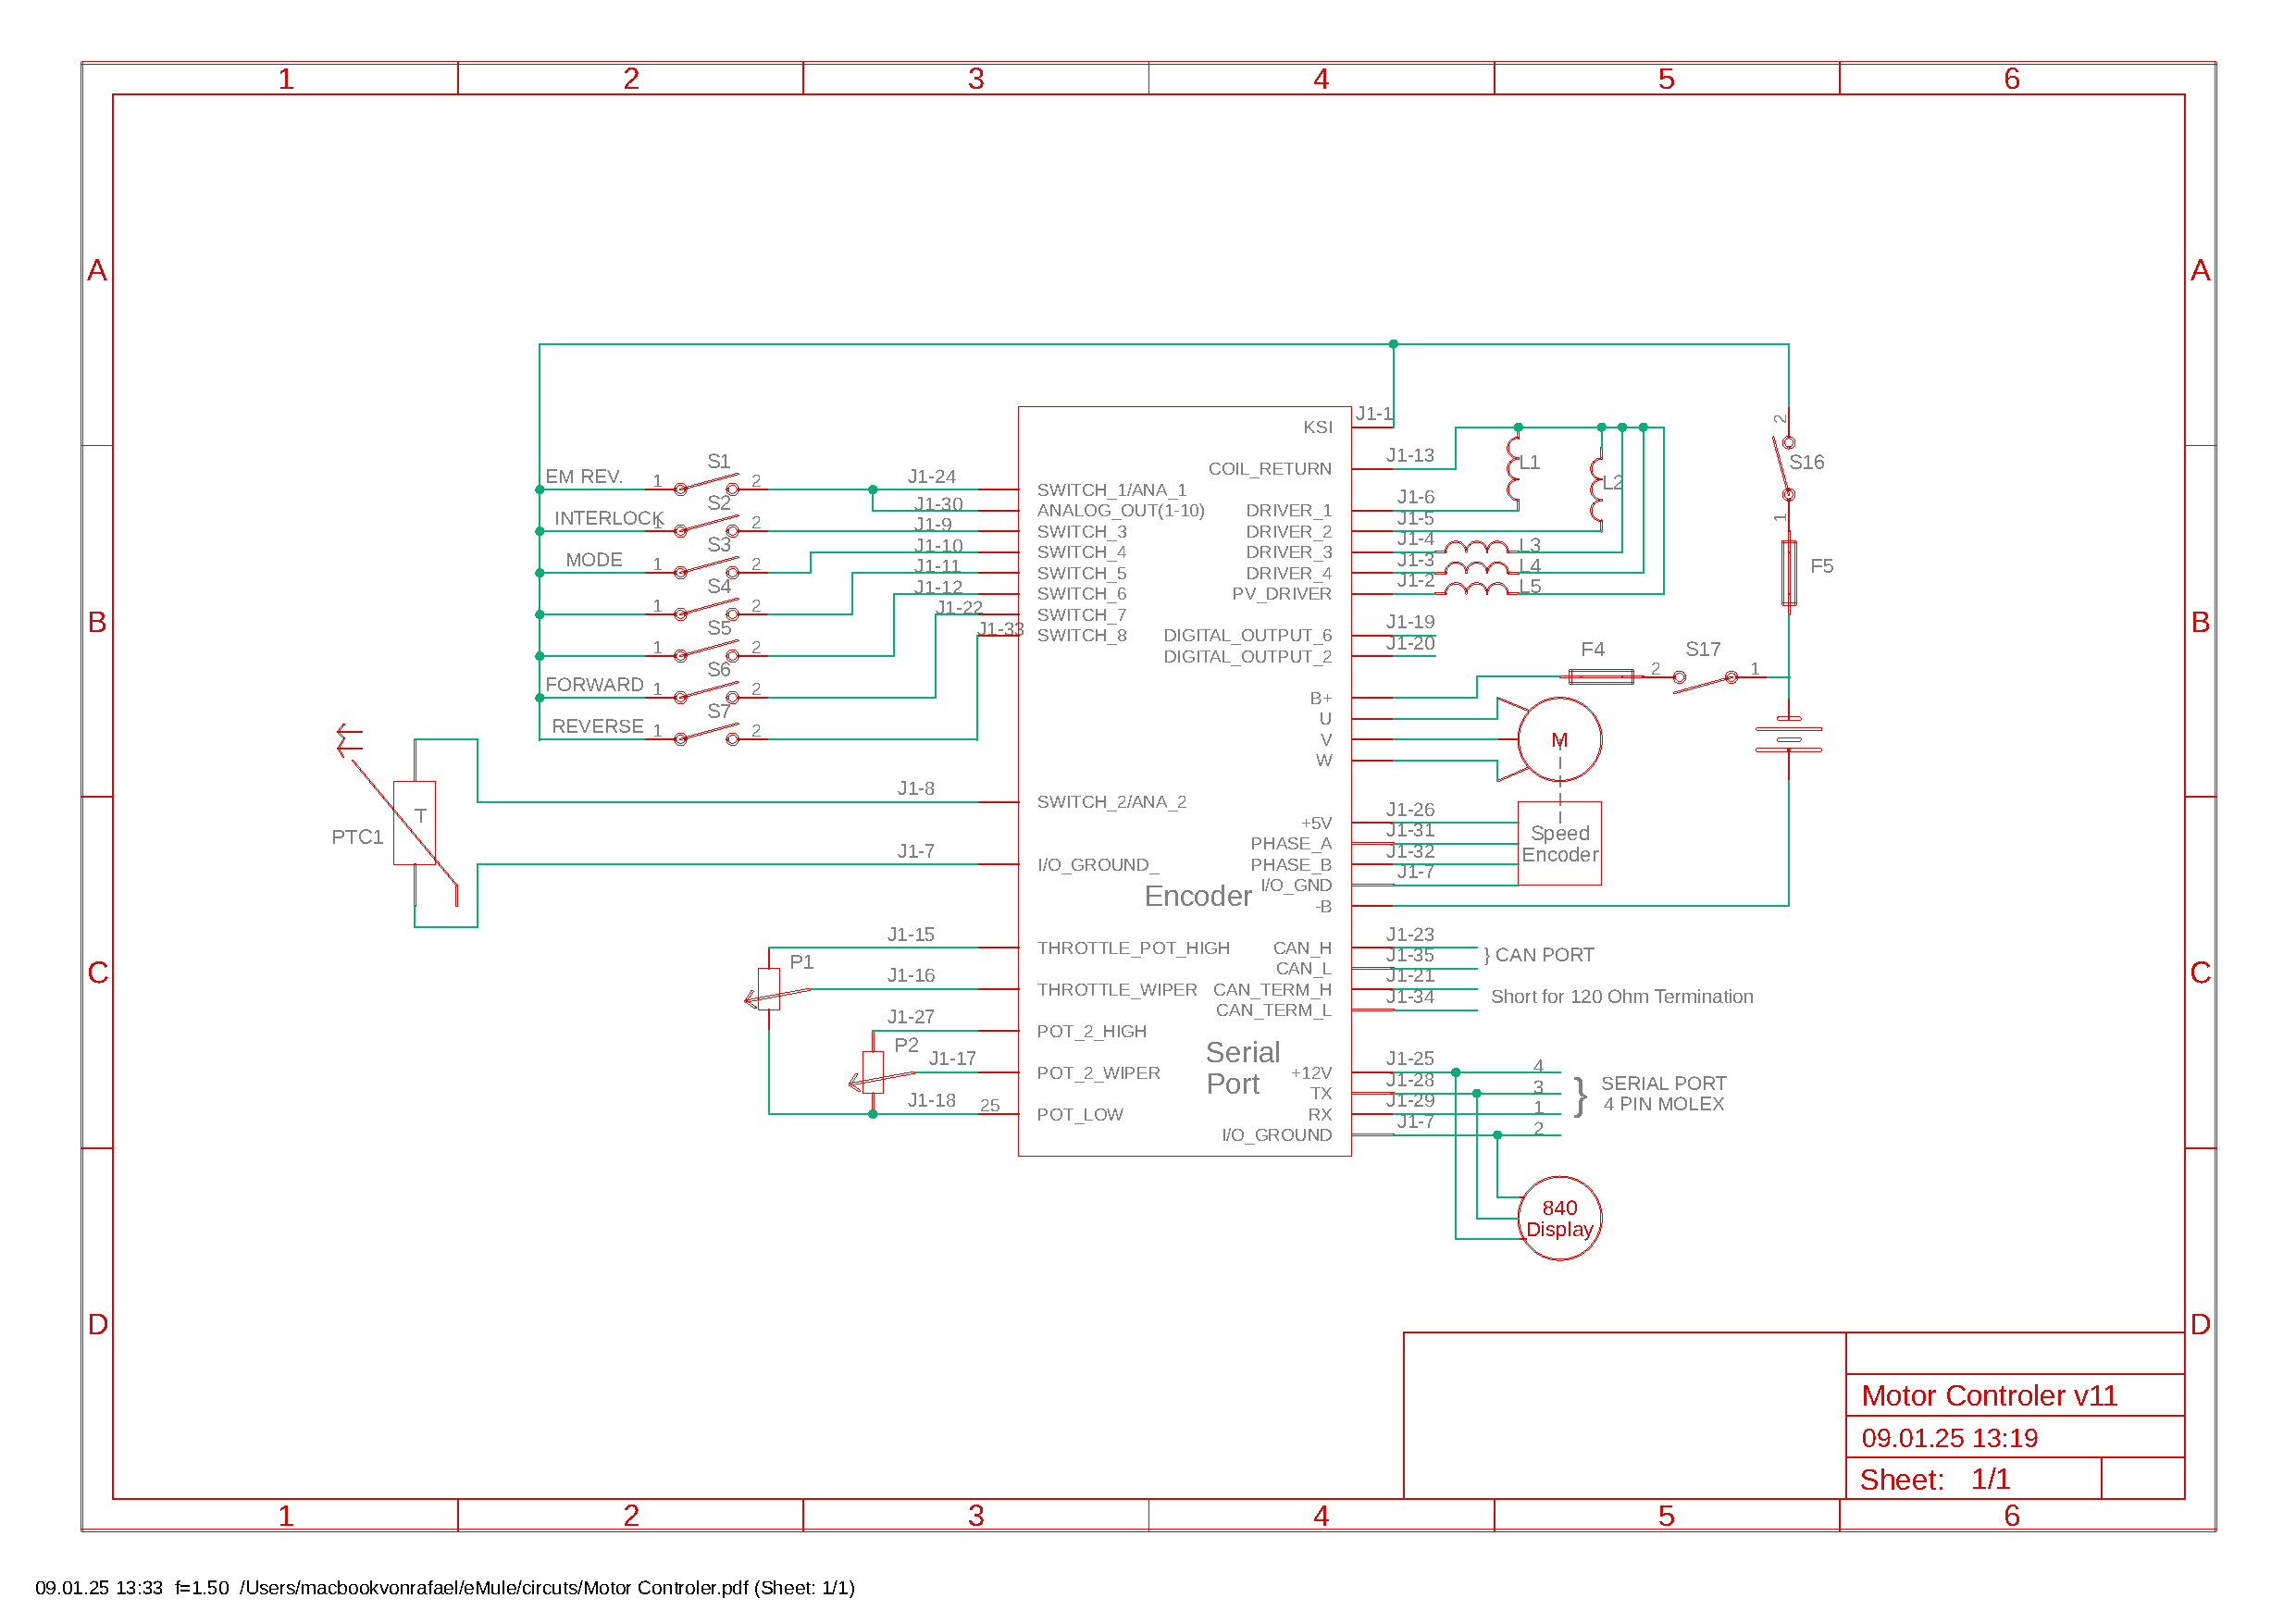
\includepdf[pages=1, fitpaper=true, pagecommand={%
	\thispagestyle{empty} % Entfernt Seitenzahlen und Kopfzeilen
	\begin{center}
		\captionof{figure}{Schaltplan des Motor Controllers} % Fügt die Caption ein
		\label{fig:motor_controller} % Für Querverweise
	\end{center}
}]{circuts/Motor Controler.pdf}
\addtocounter{page}{1} % Seitenzähler korrekt erhöhen

% Dritte PDF: LV-Onboard-Network
\section*{Stromlaufplan LV-Onboard-Netz}
Für die Erstellung des \textit{LV-Onboard-Netz} Stromlaufplans nach festgelegter Norm und aktuellem Verbaustand wird der vorliegende Plan zunächst ausgedruckt. Im ersten Schritt wird dieser Stromlaufplan systematisch auf Unstimmigkeiten, wie fehlende Verbindungen oder unklare Symbolik, überprüft. Gefundene Fehler werden im nächsten Schritt markiert und anschließend korrigiert, wobei die Einhaltung elektrotechnischer Standards gewährleistet wird. Zudem erfolgt eine Layoutanpassung zur Verbesserung der Übersichtlichkeit. Im letzten Schritt muss herausgefunden werden, nach welcher Norm der Stromlaufplan erstellt wurde. Diese Norm muss recherchiert und in die von uns gewählte DIN EN 60617 Norm \glqq übersetzt\grqq {} werden. Der überarbeitete Stromlaufplan wird abschließend mit Autodesk Fusion 360 in ein DIN-A3-Format übertragen. Dabei werden Titelblock und Legende integriert, um die Professionalität und Lesbarkeit sicherzustellen.

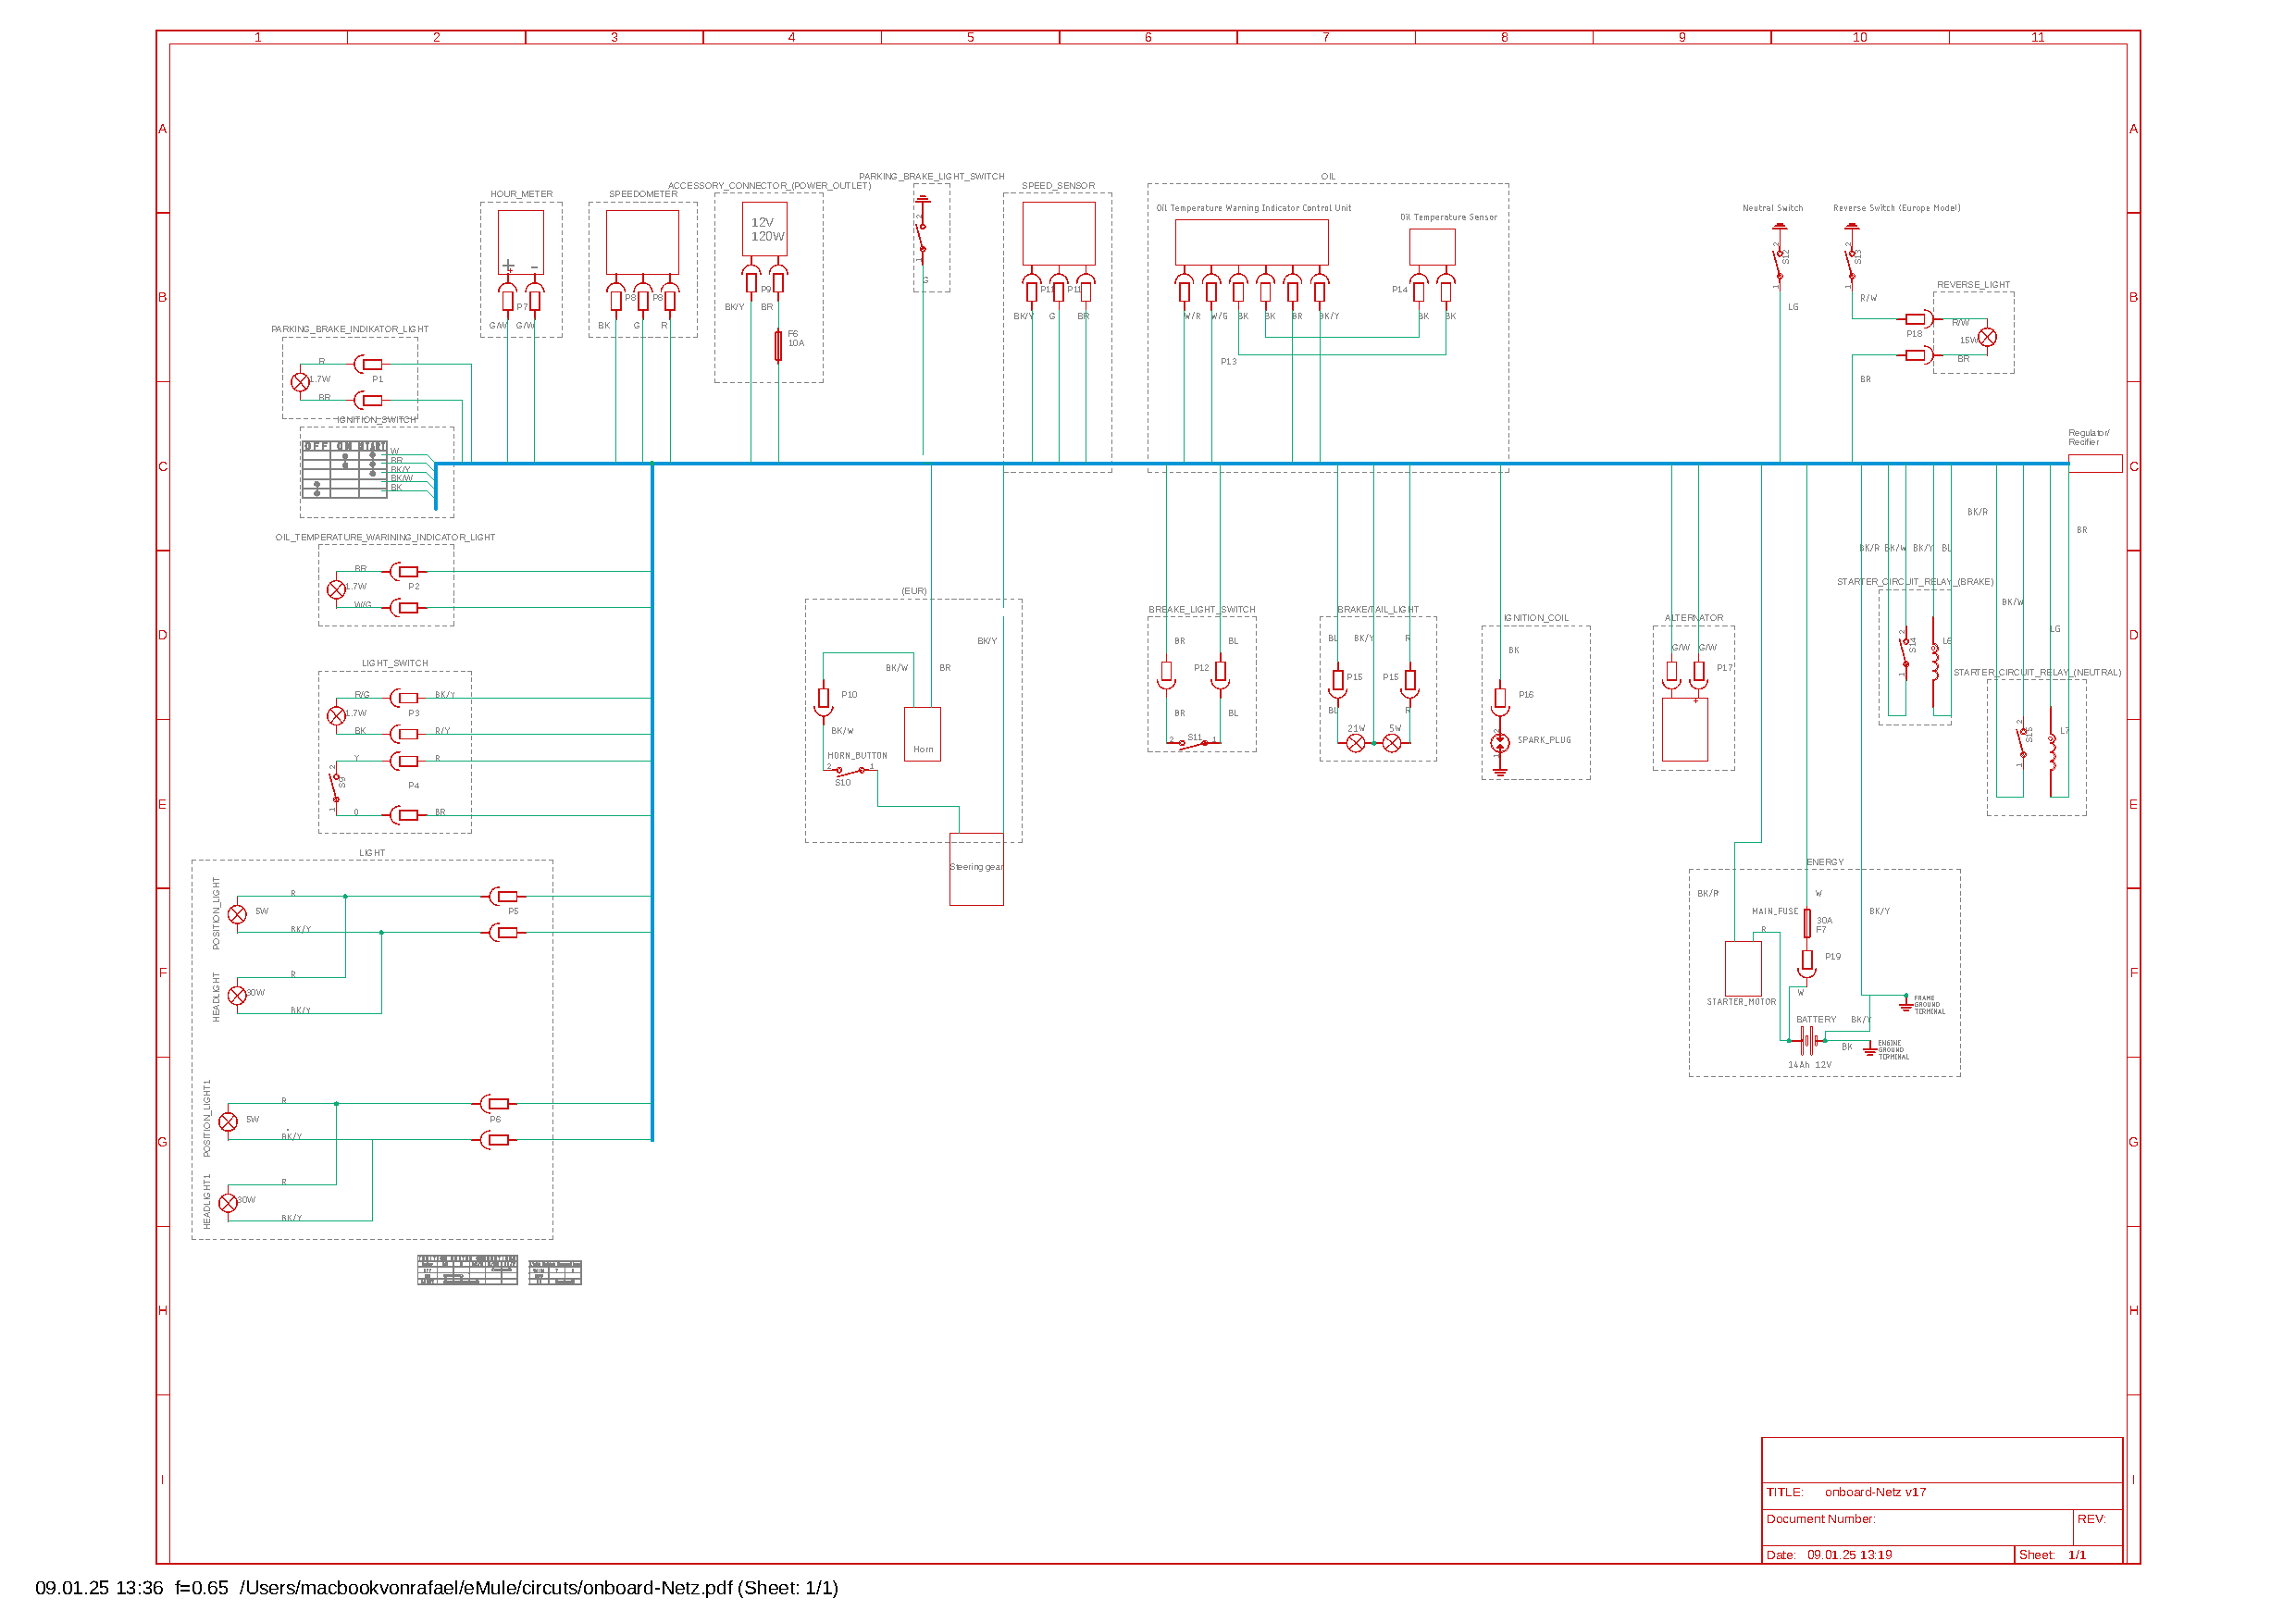
\includepdf[pages=1, fitpaper=true, pagecommand={%
	\thispagestyle{empty} % Entfernt Seitenzahlen und Kopfzeilen
	\begin{center}
		\vspace*{-2cm} % Verschiebt die Caption um 2 cm nach oben
		\captionof{figure}{Schaltplan des LV-Onboard-Netz} % Fügt die Caption ein
		\label{fig:lv_onboard_network} % Für Querverweise
	\end{center}
}]{circuts/onboard-Netz.pdf}
\addtocounter{page}{1} % Seitenzähler korrekt erhöhen

% Vierte PDF: Charger Temperature Control
\section*{Stromlaufplan Charger Temperature Control}
Für die Erstellung des \textit{Charger Temperature Control} Stromlaufplans nach festgelegter Norm und aktuellem Verbaustand wird zunächst eine händische Skizze des Systems, durch die für den Einbau zuständigen Kollegen, angefertigt und an das Dokumentationsteam weitergegeben. Im ersten Schritt wird dieser Stromlaufplan systematisch auf Unstimmigkeiten, wie fehlende Verbindungen oder unklare Symbolik, überprüft. Gefundene Fehler werden im nächsten Schritt markiert und anschließend korrigiert, wobei die Einhaltung elektrotechnischer Standards gewährleistet wird. Zudem erfolgt eine Layoutanpassung zur Verbesserung der Übersichtlichkeit. Im letzten Schritt muss die Normkonformität der Stromlaufplanskizze überprüft werden. Der überarbeitete Stromlaufplan wird abschließend mit Autodesk Fusion 360 in ein DIN-A3-Format übertragen. Dabei werden Titelblock und Legende integriert, um die Professionalität und Lesbarkeit sicherzustellen.

\includepdf[pages=1, fitpaper=true, pagecommand={%
	\thispagestyle{empty} % Entfernt Seitenzahlen und Kopfzeilen
	\begin{center}
		\captionof{figure}{Schaltplan der Charger Temperature Control} % Fügt die Caption ein
		\label{fig:charger_temperature_control} % Für Querverweise
	\end{center}
}]{circuts/Temperatursteuerung des Ladegerätes.pdf}
\addtocounter{page}{1} % Seitenzähler korrekt erhöhen

% Fünfte PDF: HV-Onboard-Network
\section*{Stromlaufplan HV-Onboard-Network}
Für die Erstellung des \textit{HV-Onboard-Network} Stromlaufplans nach festgelegter Norm und aktuellem Verbaustand wird zunächst eine händische Skizze des Systems, durch die für den Einbau zuständigen Kollegen, angefertigt und an das Dokumentationsteam weitergegeben. Im ersten Schritt wird dieser Stromlaufplan systematisch auf Unstimmigkeiten, wie fehlende Verbindungen oder unklare Symbolik, überprüft. Gefundene Fehler werden im nächsten Schritt markiert und anschließend korrigiert, wobei die Einhaltung elektrotechnischer Standards gewährleistet wird. Zudem erfolgt eine Layoutanpassung zur Verbesserung der Übersichtlichkeit. Im letzten Schritt muss die Normkonformität der Stromlaufplanskizze überprüft werden. Der überarbeitete Stromlaufplan wird abschließend mit Autodesk Fusion 360 in ein DIN-A3-Format übertragen. Dabei werden Titelblock und Legende integriert, um die Professionalität und Lesbarkeit sicherzustellen.

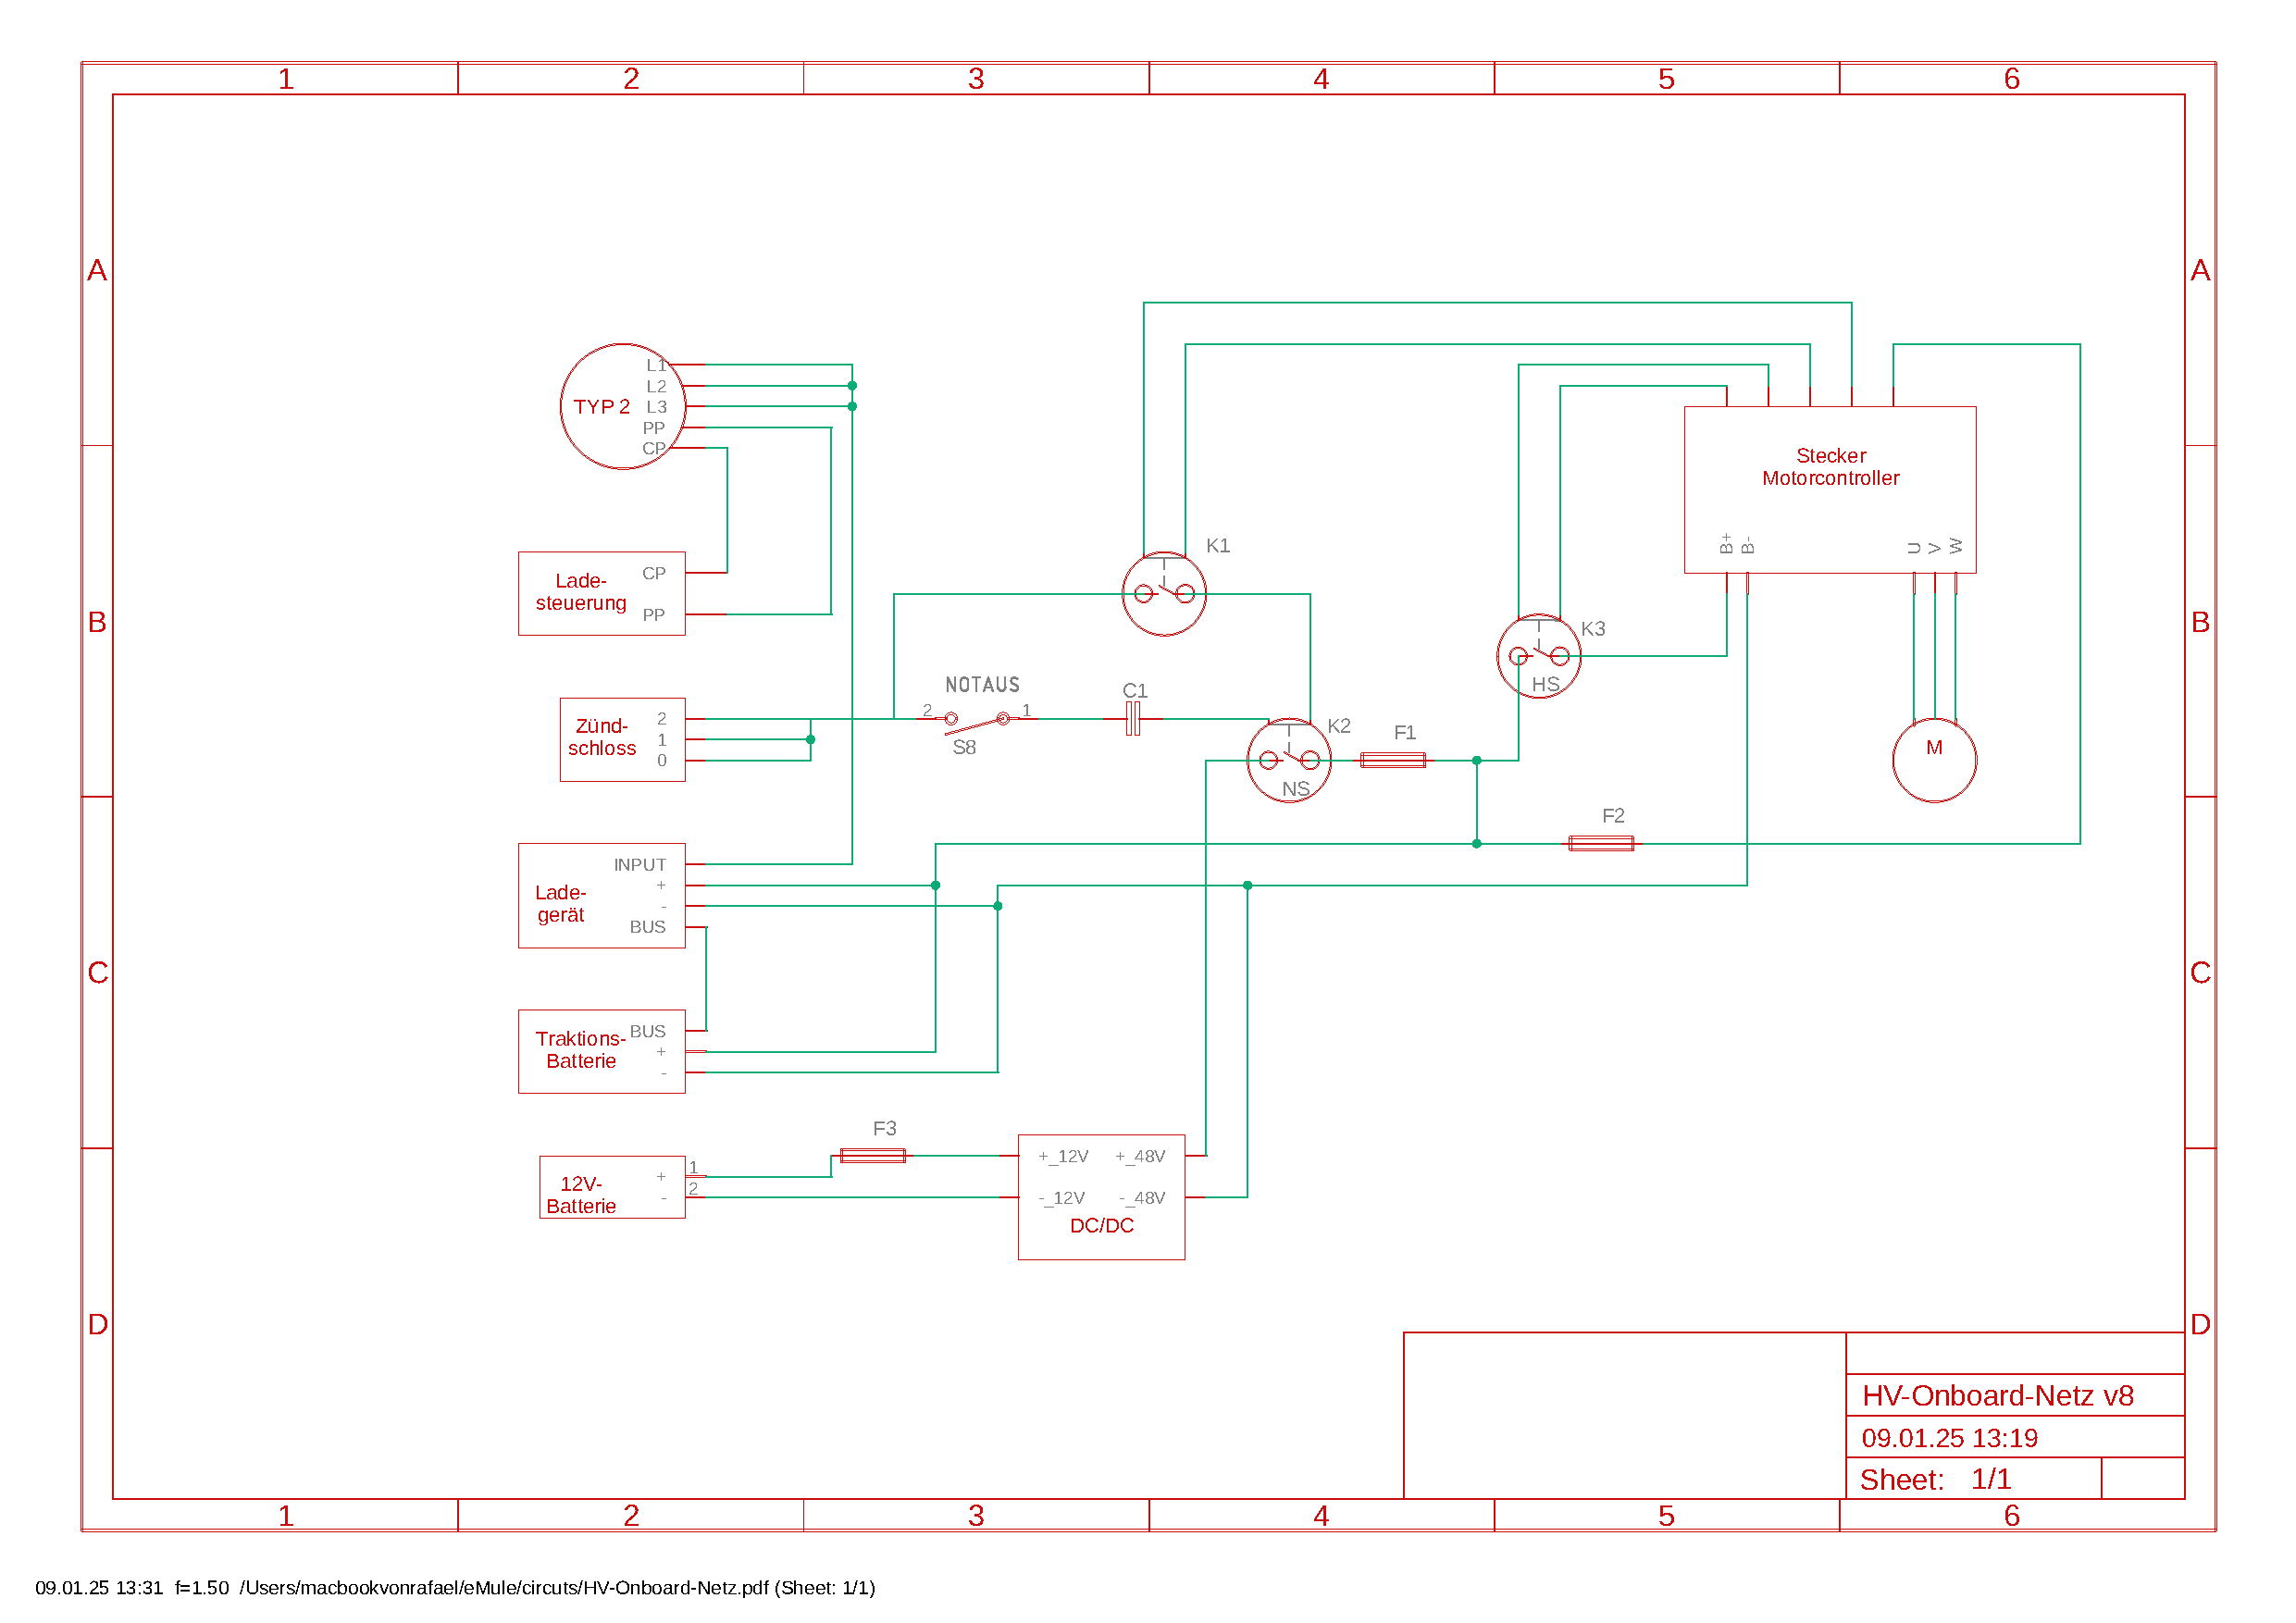
\includepdf[pages=1, fitpaper=true, pagecommand={%
	\thispagestyle{empty} % Entfernt Seitenzahlen und Kopfzeilen
	\begin{center}
		\captionof{figure}{Schaltplan des HV-Onboard-Networks} % Fügt die Caption ein
		\label{fig:hv_onboard_network} % Für Querverweise
	\end{center}
}]{circuts/HV-Onboard-Netz.pdf}
\addtocounter{page}{1}
\section*{Legende der Schaltzeichen}
In der folgenden Tabelle werden die verwendeten Schaltzeichen des Stromlaufpläne gemäß der Norm DIN EN 60617 erläutert. Diese Schaltzeichen dienen dazu, die elektrischen Komponenten und deren Verbindungen im Stromlaufplan eindeutig und standardisiert darzustellen. Die Legende bietet eine Übersicht über jene Symbole, die in den vorangegangenen Stromlaufplänenplänen verwendet werden, und erleichtert so das Verständnis der Systemarchitektur und Funktionalität der einzelnen Pläne sowie des Gesamtsystems. Dieses Verzeichnis umfasst aktuell:

\begin{multicols}{2}
	\begin{itemize}
		\item Schütz
		\item Kondensator
		\item Funkenstrecke
		\item Masse
		\item Batterie
		\item Sicherung
		\item Schalter
	\end{itemize}
	\columnbreak
	\begin{itemize}
		\item PTC-Wiederstand
		\item Potentiometer
		\item Stecker
		\item LED
		\item Spule
		\item Drei-Phasen-Motor
	\end{itemize}
\end{multicols}

Im weiteren Verlauf des Projekts kann dieses Verzeichnis beliebig um weitere Schaltzeichen ergänzt und angepasst werden.

\begin{table}[ht]
	\centering
	\resizebox{0.75\textwidth}{!}{% Verkleinert die gesamte Tabelle auf 90 % der Textbreite
		\renewcommand{\arraystretch}{1.8}
		\setlength{\tabcolsep}{15pt}
		\begin{tabular}{|m{5cm}|m{7cm}|}
			\hline
			\textbf{Symbol} & \textbf{Beschreibung} \\
			\hline
			\centering\includegraphics[width=2cm]{Legende/Schütz.png} & \centering Schütz \tabularnewline
			\hline
			\centering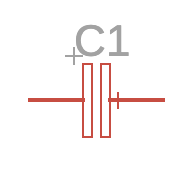
\includegraphics[width=2cm]{Legende/Kondensator.png} & \centering Kondensator \tabularnewline
			\hline
			\centering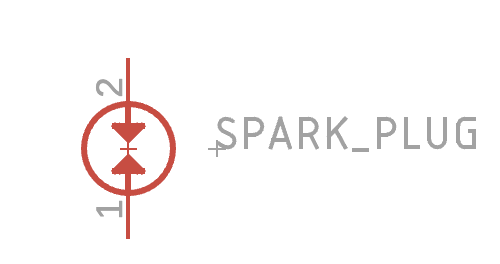
\includegraphics[width=2cm]{Legende/Funkenstrecke.png} & \centering Funkenstrecke \tabularnewline
			\hline
			\centering
\includegraphics[width=2cm]{Legende/Ground.png} & \centering Masse (Ground) \tabularnewline
			\hline
			\centering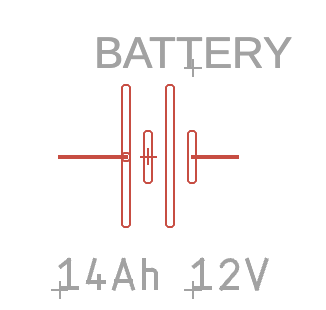
\includegraphics[width=2cm]{Legende/Batterie.png} & \centering Batterie \tabularnewline
			\hline
			\centering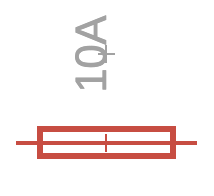
\includegraphics[width=2cm]{Legende/Sicherung.png} & \centering Sicherung \tabularnewline
			\hline
			\centering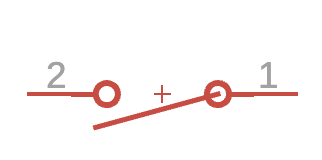
\includegraphics[width=2cm]{Legende/Schalter.png} & \centering Schalter \tabularnewline
			\hline
			\centering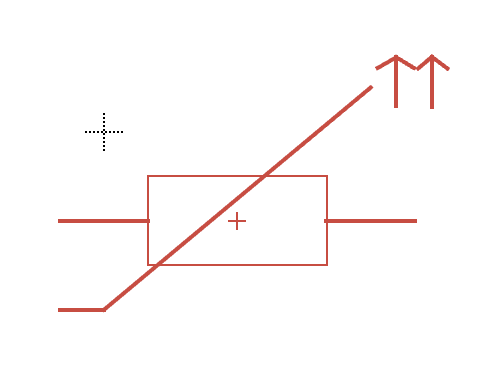
\includegraphics[width=2cm]{Legende/PTC-Widerstand.png} & \centering PTC-Widerstand \tabularnewline
			\hline
			\centering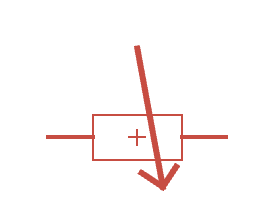
\includegraphics[width=2cm]{Legende/Potentiometer.png} & \centering Potentiometer \tabularnewline
			\hline
			\centering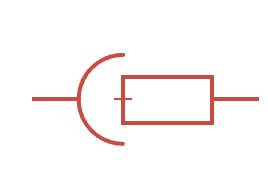
\includegraphics[width=2cm]{Legende/Stecker.png} & \centering Stecker \tabularnewline
			\hline
			\centering
\includegraphics[width=2cm]{Legende/LED.png} & \centering LED \tabularnewline
			\hline
			\centering
\includegraphics[width=2cm]{Legende/Spule.png} & \centering Spule \tabularnewline
			\hline
			\centering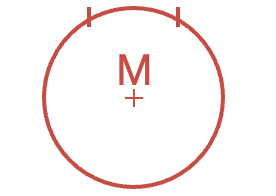
\includegraphics[width=2cm]{Legende/3 Phasen Motor.png} & \centering Drei-Phasen-Motor \tabularnewline
			\hline
	\end{tabular}}
	\caption{Legende der Symbole}
	\label{tab:legende}
\end{table}